\documentclass[tikz,border=4pt,11pt]{standalone}
\usepackage{amsmath}
\definecolor{ink}{RGB}{42,52,64}
\definecolor{first}{RGB}{146,79,26}
\definecolor{second}{RGB}{26,99,111}

% The combinatorial model for lambda = (3,3,2,1).
% Left: the Ferrers diagram; the board of squares B (boxes (1,1), (1,2),
%   (2,1), the northwest corners of 2x2 squares) is shaded, and the placement
%   {(1,2),(2,1)} is drawn as two rooks.
% Right: the Motzkin path U H D H drawn downwards, with the vertex after step j
%   level with row j of the diagram.  The path is positive after steps 1 and
%   2 (filled vertices) and at height zero after step 3 (open vertex), so
%   rooks are allowed in rows 1 and 2 only.  The pair contributes
%   y x_1 x_2 to the gamma polynomial.

\begin{document}
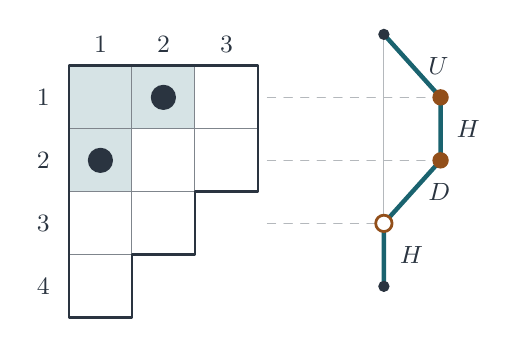
\begin{tikzpicture}[x=.8cm,y=.8cm,text=ink,line cap=round,line join=round]
  % ---------- diagram and board ----------
  \foreach \j/\c in {1/1,1/2,2/1}
    \fill[second!18] (\c-1,-\j) rectangle (\c,-\j+1);
  \foreach \j/\l in {1/3,2/3,3/2,4/1} {
    \foreach \c in {1,...,\l} {
      \draw[ink!60,line width=.4pt] (\c-1,-\j) rectangle (\c,-\j+1);
    }
  }
  \draw[ink,line width=1pt] (0,0) -- (3,0) -- (3,-2) -- (2,-2) -- (2,-3)
    -- (1,-3) -- (1,-4) -- (0,-4) -- cycle;
  \foreach \j/\c in {1/2,2/1} \fill[ink] (\c-.5,-\j+.5) circle (.2);
  \foreach \j in {1,...,4} \node[font=\small,anchor=east] at (-.15,-\j+.5) {$\j$};
  \foreach \c in {1,2,3} \node[font=\small,anchor=south] at (\c-.5,.05) {$\c$};

  % ---------- Motzkin path, drawn downwards ----------
  \def\X{5}
  \draw[ink!35] (\X,.5) -- (\X,-3.5);
  \foreach \j/\h in {1/1,2/1,3/0}
    \draw[ink!35,dashed] (3.15,-\j+.5) -- (\X+.9*\h,-\j+.5);
  \draw[second,line width=1.6pt] (\X,.5) -- (\X+.9,-.5) -- (\X+.9,-1.5)
    -- (\X,-2.5) -- (\X,-3.5);
  \fill[ink] (\X,.5) circle (.09);
  \fill[ink] (\X,-3.5) circle (.09);
  \fill[first] (\X+.9,-.5) circle (.13);
  \fill[first] (\X+.9,-1.5) circle (.13);
  \fill[white] (\X,-2.5) circle (.13);
  \draw[first,line width=1pt] (\X,-2.5) circle (.13);
  \node[font=\small,anchor=west] at (\X+.55,0) {$U$};
  \node[font=\small,anchor=west] at (\X+1,-1) {$H$};
  \node[font=\small,anchor=west] at (\X+.55,-2) {$D$};
  \node[font=\small,anchor=west] at (\X+.1,-3) {$H$};
\end{tikzpicture}
\end{document}
